\documentclass{article}


\usepackage{arxiv}

\usepackage[utf8]{inputenc} % allow utf-8 input
\usepackage[T1]{fontenc}    % use 8-bit T1 fonts
\usepackage{hyperref}       % hyperlinks
\usepackage{url}            % simple URL typesetting
\usepackage{booktabs}       % professional-quality tables
\usepackage{amsfonts}       % blackboard math symbols
\usepackage{nicefrac}       % compact symbols for 1/2, etc.
\usepackage{microtype}      % microtypography
\usepackage{lipsum}
\usepackage{graphicx}
\usepackage{caption}
\usepackage{subcaption}
\usepackage{lipsum}
% \graphicspath{ {./images/} }
\usepackage{mathtools,amssymb}
\usepackage{tablefootnote}

\usepackage{float}
\floatstyle{plaintop}
\restylefloat{table}

\title{Identify the Similarity of Glyphs using a Siamese Network by Triplet Loss and Contrastive loss \\
{\sl \Large IFN680 Assignment 2}}


\author{
 Zhipeng He \\
  School of Information Systems\\
  Queensland University of Technology\\
  \textit{n10599070} \\
  \texttt{zhipeng.he@connect.qut.edu.au} \\
}

\begin{document}
\maketitle

\vspace{5em}

\section{Introduction}

The problem of most recognition systems based on deep neural network is their performance is subjected to projective transformations that simulate changes in the camera perspective. This is not robust when the perspective of the camera changes dramatically. The category of an object in an image is the category of an object could be various to viewpoint changes. This causes an issue for an automated system to recognize sea species such as manta rays\footnote{https://www.mantatrust.org/idthemanta}. Siamese network, based on Convolutional Neural Network (CNN), is a good approach to solve this problem, which can learn to differentiate between two input images. In this report, it will performance the experiments by a Siamese network by Triplet Loss and Contrastive loss function to categorise images which have been geometrically transformed. The objective of the experiments is to determine whether an image can be correctly classified into it’s equivalent class by comparing two images. The model can classify equivalence classes which are different images show the same object from various observation point.


\section{Methodology}

\subsection{One-shot learning}

While trying to achieve human-like capabilities, machine learning was very effective and successful in various applications such as web search, fraud detection, text generation, and speech and image recognition. However, these algorithms often fail when stressed on making predictions about data that has less supervised information. One particularly interesting task is image classification under the restriction on size of data. i,e we might have only one example of each possible class before we make a prediction. This is called one-shot learning. Where the learning algorithm looks at an image once and learns features to distinguish it from rest.

The problem of one-shot learning can be directly addressed by developing domain-specific features
or inference procedures which possess highly discriminative properties for the target task. As a result,
systems which incorporate these methods tend to excel at similar instances but fail to other robust
solutions that may be generally applied to other types of problems. In this paper, we present a novel
approach which limits assumptions on the structure of the inputs while automatically acquiring features
which enable the model to generalize successfully from few examples. We build upon the deep learning
framework, which uses many layers of non-linearities to capture invariance to transformation in the
input space, usually by leveraging a model with many parameters and then using a large amount of data
to prevent overfitting. These features are very powerful because we are able to learn them without
imposing strong priors, although the cost of the learning algorithm itself may be considerable.

\subsection{Siamese networks}

A Convolutional Neural Network (CNN) is a class of deep, feed-forward artificial neural networks most commonly applied to analyzing visual imagery. The architecture of these networks was loosely inspired by biological neurons that communicate with each other and generate outputs dependent on the inputs. Though work on CNNs started in the early 1980s, they only became popular with recent technology advancements and computational capabilities that allow the processing of large amounts of data and the training of sophisticated algorithms in a reasonable amount of time. Some of the applications of CNNs include AI-based virtual assistant, automatic photo tagging, video labeling, and self-driving cars.

Siamese networks are a special type of CNN-based neural network architecture. Instead of a model learning to classify its inputs, the neural networks learns to differentiate between two inputs. It learns the similarity between them. It is usually used for performing verification, identification, or recognition tasks, the most popular examples being face recognition and signature verification.

\subsection{Subnetwork}

The identical subnetwork of siamese network also belongs to a type of CNN networks. Based on the previous research \cite{koch2015siamese}, the subnetwork is designed as following:

\begin{itemize}
  \item Layer 0: An input layer
  \item Layer 1: A 2D-convolution layer with 64 filters and pool sizes of $10\times10$ by `relu' function
  \item Layer 2: A 2D-maxpooling layer with pool sizes of $2\times2$
  \item Layer 3: A 2D-convolution layer with 128 filters and pool sizes of $7\times7$ by `relu' function
  \item Layer 4: A 2D-maxpooling layer with pool sizes of $2\times2$
  \item Layer 5: A 2D-convolution layer with 128 filters and pool sizes of $4\times4$ by `relu' function
  \item Layer 6: A 2D-maxpooling layer with pool sizes of $2\times2$
  \item Layer 7: A 2D-convolution layer with 256 filters and pool sizes of $4\times4$ by `relu' function
  \item Layer 8: A flatten layer
  \item Layer 9: A fully connected (dense) layer with 4096 units

\end{itemize}

Fig.~\ref{subnetwork} shows the structure of subnetwork. It shows that each subnetwork is used to processing one image at one time. Hence, siamese networks always require more than two subnetworks for constructing a full model.

\begin{figure}[b]
  \centering
  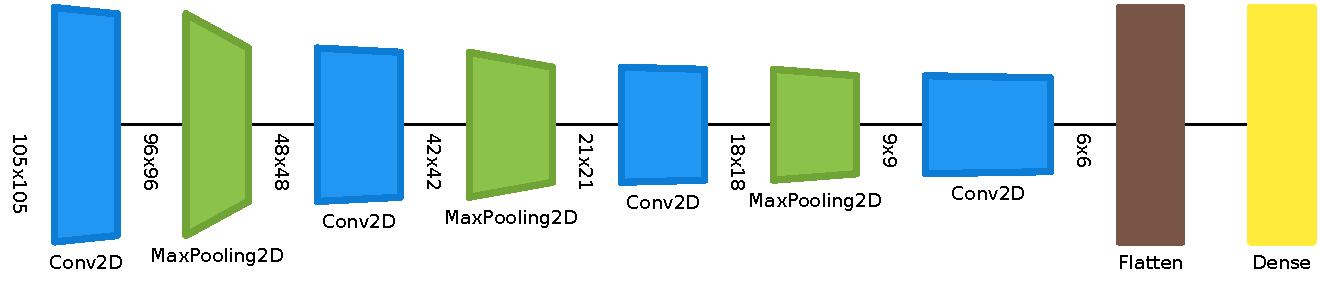
\includegraphics[width=\textwidth]{image/graph.pdf}
  \caption{The subnetwork architecture adapted from~\cite{koch2015siamese} }\label{subnetwork}
\end{figure}

\subsection{Loss Functions}

The structures of full siamese networks are various if using different predictive methods. In practical, it is depending on the usage of loss functions. There are two loss function using in this experiment, which are contrastive loss function and triplet loss function. Here, two popular loss functions are introduced, which are contrastive loss function and triplet loss function.


\paragraph{Contrastive loss function}The aim of the training algorithm is to minimize the distance between a pair of images from the same equivalence class while maximizing the distance between a pair of images from different equivalence classes. The input images $P_i$ and $P_j$ are fed to the twin sub-networks to produce two vector representations $f(P_i)$ and $f(P_j)$ that are used to calculate a proxy distance. The training of a Siamese network is done
with a collection of positive and negative pairs. Learning is performed by optimizing a contrastive
loss function, which is defined as:

\begin{equation}
  \mathcal{L}_c (P_i,P_j)=
  \begin{cases}
  \frac{1}{2} D(P_i,P_j)^2, & \text{if } y_{i,j}=0 \\
  \frac{1}{2} \max(0,m-D(P_i,P_j))^2, & \text{if } y_{i,j}=1
  \end{cases}
\end{equation}

where $D(P_i, P_j)$ is the euclidian distance between $f(P_i)$ and $f(P_j)$. The margin $m > 0$ determines
how far the negative pair should be pushed apart.


\paragraph{Triplet loss function} The Triplet Loss helps to learn which features, represented by the embedding
vectors, differentiate samples of different images. It generates close embedding vectors when the inputs belong to the same species and, at the same time, keep them away from vectors representing other species, considering a Euclidean vector space. In this way, we hope that the new vector representation would make the classes more easily separable. It can be defined as:
 

\begin{equation}
  \mathcal{L}_h= \sum_{i=1}^N \max(0, m+D(P_i^a,P_i^+)^2-D(P_i^+,P_i^-)^2)
\end{equation}

where $P_i^a$ is an anchor input, $P_i^+$ is a positive input of the same class as $P_i^a$, $P_i^-$ is a negative input of a different class from $P_i^a$, $m > 0$ is a margin between positive and negative pairs.

Based on the previous two loss functions, two full structure siamese networks (shown in Fig,\ref{loss}) can be used in this report. 

\begin{figure}[!p]
  \centering
  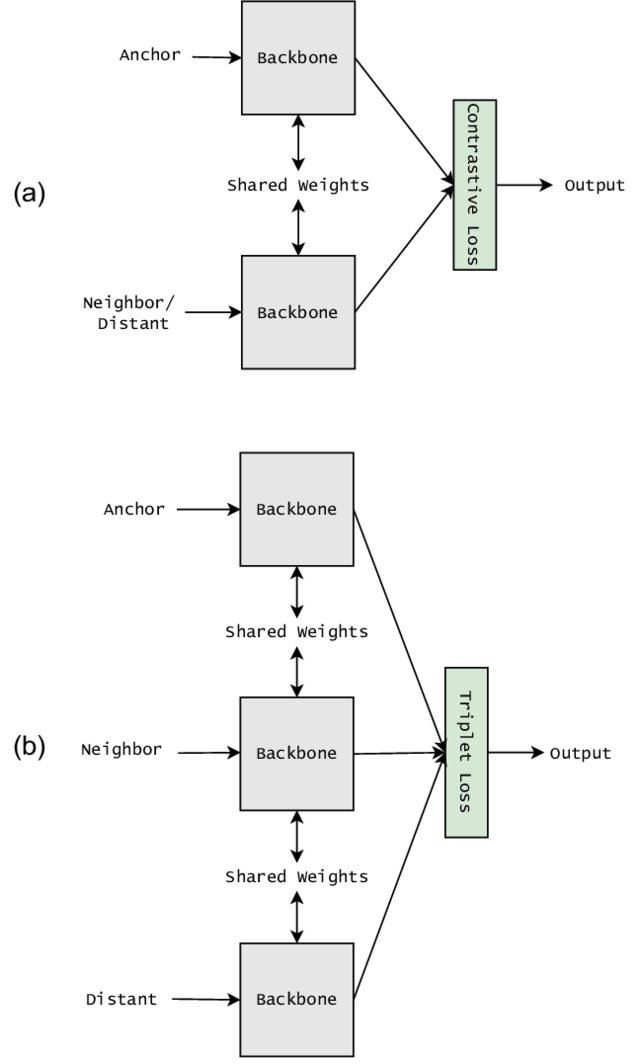
\includegraphics[width=0.5\textwidth]{image/loss-function.jpg}
  \caption{Siamese networks based on contrastive loss and triplet loss function~\cite{ghojogh2020fisher}.}\label{loss}
  \bigskip
  
    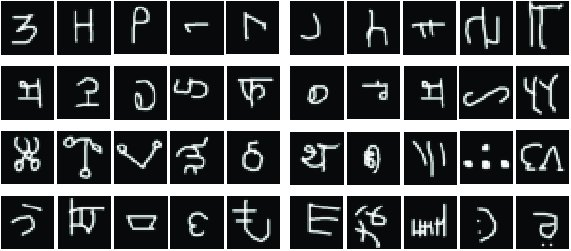
\includegraphics[width=0.8\textwidth]{image/Example-images.jpg}
  \caption{Some example images in omniglot.}\label{omniglot}
\end{figure}



\section{Experiment settings}

\subsection{Dataset}

Omniglot is a dataset of handwritten characters from 50 different alphabets. The dataset was developed to study how humans and machines perform one-shot learning, which is the ability to learn a new concept from just a single example. The domain of handwritten characters provides a large set of novel, high-dimensional concepts that people learn and use in the real world. The omniglot dataset contains 1623 character classes from 50 alphabets (real and fictional) and 20 hand-written, gray-scale, 105 × 105 pixel examples of each. Fig.~\ref{omniglot} shows some example images from omniglot.

\paragraph{Data split} During the preprocessing stage, all images have been shuffled and they will be split into train and test set by \texttt{tfds.load()} automatically. Additionally, 20\% of the data from the training set is used as validation split to avoid the overfitting or underfitting in the learning phrase. For splitting validation set, it is processed by my own functions.

\subsection{Metrics}

Although the tasks in this report are not the classical classification problems, the experiment will utilize accuracy metric. It represents the proportion of all correct classifications in all prediction. The calculation of the accuracy is done by own function, since the output of proposed deep learning models are designed as the tensors of each processed images and the prediction step in evaluation will also be done by own functions.

\subsection{Implementation details}

The experiments were performed on a server with Windows 10 Operation System and its hardware contained 3.8 GHz AMD Ryzen 3900X CPU having 64 GB RAM and one single NVIDIA RTX A4000 GPU with 16 GB Memory. Here are some key ideas for implementation:

\begin{itemize}
  \item The deep neural networks are implemented by TensorFlow 2.5 Library in Python.
  \item The constructed models are trained by a SGD optimiser with a learning rate of 0.01 (default learning rate) for all event logs in the experiments.
  \item The number of epoch is set to 20 with batch size of 256.
  \item When evaluating the models, the prediction of each splits are done by own functions, since the output of proposed deep learning models are designed as the tensors of each processed images. 
\end{itemize}

\section{Model performance}

\subsection{Contrastive loss-based model}

Fig.\ref{Siamese-network-with-contrastive-loss} shows the relationship between loss and time for siamese networks based on contrastive loss function.

\begin{figure}[!ht]
  \centering
  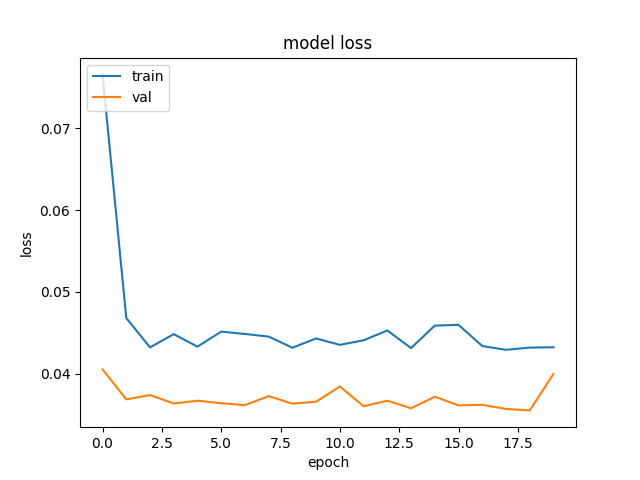
\includegraphics[width=0.7\textwidth]{image/Siamese-network-with-contrastive-loss.png}
  \caption{Loss vs. time for contrastive loss-based model.}\label{Siamese-network-with-contrastive-loss}
\end{figure}

The results of evaluation on the training split, test split and both training and test split are shown in Table 1 below.

\begin{table}[!ht]
\center

\begin{tabular}{llll}
\hline
            & True & False & Accuracy \\ \hline
Train split &  9256    &   384    & 0.9602        \\
Test split  &   6233   &    357   & 0.9543         \\
Train and test split   &  15490   &   740    &   0.9458       \\ \hline
\end{tabular}
\caption{Results of evaluation for contrastive loss-based model.}
\end{table}

From the above results, loss-based siamese networks achieve an excellent performance.


\subsection{Triplet loss-based model}

The triplet loss function passed the test and the siamese networks for triplet loss also build successfully. However, the errors in splitting datasets for triplet loss-based model make the training and evaluation of triplet loss-based model unsuccessfully. Thus, I cannot get the results of triplet loss-based siamese networks.


\bibliographystyle{unsrt}
\bibliography{references}  %%% Remove comment to use the external .bib file (using bibtex).


\end{document}
